%\section{Experiment Setup}

%We will begin by measuring the baseline traffic from the smart speaker in a silent environment. This should allow us to identify the regular traffic patterns of the smart speaker when it is not transmitting voice data. %We will then test several basic pre-recorded commands with the smart speaker to identify the basic traffic signature of the speaker when it is transmitting voice data.
%
%Once we have baseline traffic patterns we will begin more detailed measurements. We will test pre-recorded commands of varying lengths many times, to establish correlations between recording length and traffic speed and/or duration. We will then repeat these tests in the presence of several different forms of background noise, including at least podcasts, music, and discussion among ourselves. %We will not perform any tests in public environments to avoid any possible ethical considerations.
%
%To determine how the speaker decides to terminate its recording, we will use several different pathological commands. We will use incomplete commands, very long commands, and commands spoken very unclearly. By correlating the traffic patterns of these commands to the more normal commands previously measured, we hope to calculate the rough length of time the recording lasts.
%
%We will obtain whatever information we can from the cloud (e.g. through an app or API) to compare such information to our traffic pattern analysis and determine whether they match within whatever margin of error we can achieve. We will also test the behavior of the speaker in noisy environments without any commands being given to determine the rate of false recordings.
%
%\subsection{Devices}
%Our main device for testing will be the Amazon Echo, as it is the most popular smart speaker.
%
%If available, we would also like to test the Apple HomePod, as Apple places a much greater emphasis on security and privacy than its competitors.

\section{Experiment}

We ran some experiments on Alexa and used Wireshark to see if Alexa recorded consumer's voice more than it should.

\subsection{Monitoring Set Up}
\label{sec:expr:set-up}

In order to catch the packets that were sent out by Alexa to the Amazon cloud server, we set up a WiFi router on a desktop server and connected the Echo to it. We run Wireshark~\cite{wireshark} on the desktop server to capture all the packets to and from the Echo speaker.

Since we cannot directly examine the contents of the packets sent to and from the Echo, as they are all encrypted by TLS, we instead must examine coarser-grained information, like packet count, packet sizes, server IP addresses, and packet timing information. Since most of this kind of coarser-grained information is subject to variation based on network conditions, and the voice data itself is subject to variation based on environmental noise, we opt to repeat all of our experiments many times (10s to 100s) to allow us to draw statistical conclusions. 

To ensure the repeatability of such experiments, we synthesize all our voice commands and play them to the Echo using the desktop server. We also use it record any response that the Echo may give, which allows us to gather all relevant data for our experiments on a single, centralized platform. Each experiment consists of some number of different voice commands that we iterate through throughout the experiment. We leave 30~s to a minute between each command to allow the Echo to reset, and after reaching the end of our set of commands, we loop back to the beginning. We perform each experiment overnight in the office, to remove any extra human noise and ensure that the Echo only responds to the commands we provide it. We interleave the commands that we are testing to make sure that any variation throughout the night due to conditions we cannot account for affect each of the commands equally.

To make analysis easier, we use the desktop server to inject markers into the Wireshark packet capture at critical moments. This allows the analysis code to read only the single Wireshark capture and still obtain all necessary information. In particular, the desktop server pings four different predefined locations (\textit{e.g.}, 8.8.8.8) at four specific times: when the command starts playing, when the command stops playing, when Alexa's response begins, and when Alexa's response ends.

\subsection{Analysis Techniques}


After an overnight run of an experiment, we programmatically divide the Wireshark capture into experiment frames (individual command trials). We define these frames using the ping packets generated by the desktop server; the extent of each frame spans from the start of the voice command to the start of Alexa's response. This captures all the data sent by the Echo to the Amazon servers and the response from the Amazon servers back to the Echo, since we know that such a response must be complete by the time the Echo speaks that response.

\begin{figure}[!t]
    \centering
    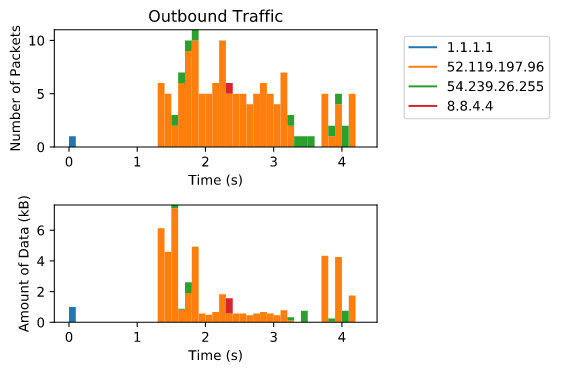
\includegraphics[width=\linewidth]{sample_hist_out.png}
    \caption{On top, time histogram of the number of packets sent from the Echo, sorted by destination IP address. On bottom, time histogram of total data sent from the Echo, sorted in the same way. The blue and red bars do not indicate real traffic, but rather mark the start and end of the command given to the Echo, as discussed in Section~\ref{sec:expr:set-up}. The time histogram ends at the moment the Echo begins its reply. The orange bars are those of the Alexa server, in this case, as they constitute by far the most data.}
    \label{fig:example_frame}
\end{figure}

The Echo communicates with many different servers for background tasks, and even a couple different servers as part of processing a command. As shown in Fig.~\ref{fig:example_frame}, though, the Echo sends the majority of its data to a single IP address, namely the Amazon server handling the Alexa request. For each frame, we choose to only count the data going to this server, as it provides the most consistent metric to compare across. The precise identity of the Alexa server changes fairly frequently, so in the course of our analyses we used two different methods to identify the server in each frame: (1) we manually inspected many packet data time histograms (as in Fig.~\ref{fig:example_frame}) to create a whitelist of Alexa serves, and (2) we simply chose the IP address in each frame that had the most data sent to it. Both methods gave very similar results, so we used the latter for most analyses, as it was more automated.

Some of the frames had much more data sent in them than others did, and inspection of their time histograms generally revealed that this was due to unusual traffic patters clearly not related to our commands (perhaps background updates or other such maintenance). These outliers needed to be filtered, as in some cases they were so high as to completely change the mean and standard variation of the entire data set. To filter such outliers, we decided to use the IQR (inter-quartile range) method to remove them. The IQR is defined as the difference of the 3rd quartile value and the 1st quartile value, and we filter any value that is more than 1.5*IQR higher than the 3rd quartile value or 1.5*IQR lower than the 1st quartile value. In other words, we keep a value $x$ only if $Q1 - 1.5*IQR < x < Q3 + 1.5*IQR$. We chose this method because of its high robustness to large outliers.

We choose to count only the data sent in TLS packets, as the Echo encrypts all of its traffic, and so any other packets are only handshakes, DNS requests, or other such administrative packets. We are careful to count only the size of the actual TLS payload, and not any of the header bytes, so as to ensure the most accurate accounting possible.



